
% This LaTeX was auto-generated from an M-file by MATLAB.
% To make changes, update the M-file and republish this document.

\documentclass{article}
\usepackage{graphicx}
\usepackage{color}

\sloppy
\definecolor{lightgray}{gray}{0.5}
\setlength{\parindent}{0pt}

\begin{document}

    
    
\section*{SEM1D}

\begin{par}
Spectral Element Method solver for the 1D wave equation
\end{par} \vspace{1em}
\begin{par}
$$u_{tt} = u_{xx} + F(t)\times\delta(x-xs)$$
\end{par} \vspace{1em}
\begin{par}
with a time dependent point source F(t) located at \texttt{x=xs}, zero initial conditions and Dirichlet boundary conditions.
\end{par} \vspace{1em}
\begin{par}
This script is intended for tutorial purposes.
\end{par} \vspace{1em}
\begin{par}
Jean-Paul Ampuero	\ensuremath{<}mailto:ampuero@erdw.ethz.ch ampuero@erdw.ethz.ch\ensuremath{>}
\end{par} \vspace{1em}

\subsection*{Contents}

\begin{itemize}
\setlength{\itemsep}{-1ex}
   \item STEP 1: SET PARAMETERS
   \item STEP 2: INITIALIZATION
   \item STEP 3: SOLVER
\end{itemize}


\subsection*{STEP 1: SET PARAMETERS}

\begin{verbatim}
L=10;           % domain size
NEL = 10;       % number of elements
P = 6;          % polynomial degree
CFL = 0.86;     % stability number (<=0.86)
NT = 1000;      % number of timesteps
Fx = 5;         % location of point source (required if F_IS_WAVE=0)
Ff0 = 0.25;     % fundamental frequency of the source
OUTx  = (0:L/NEL:L)'; % output receivers at these locations
\end{verbatim}


\subsection*{STEP 2: INITIALIZATION}

\begin{verbatim}
%-- Build the "macro-mesh":
% The domain [0,L] is divided into NEL non overlapping elements
% The elements are defined by their "control nodes" X
X = (0:NEL)'*L/NEL;

%-- Build the SEM grid:
% SEM is a high-order method, each element of the macro-mesh
% contains a spectral sub-grid of Gauss-Lobato-Legendre (GLL) internal nodes
NGLL = P+1; 				% = number of GLL nodes per element
[iglob,coor,nglob] = mesh1d(X,NGLL);	% creates the SEM grid
% Look at the outputs in "help mesh1d".
% You may be wondering what are "global" and "local" numberings.
% Let's take an example. Consider a mesh of 3 elements with index e = 1 to 3
%
%X(1)                      X(2)                      X(3)                      X(4)
% |----------- 1 -----------|----------- 2 -----------|----------- 3 -----------|
% :                         :                         :                         :
% Let's assume P=4 (NGLL=5). Each element is provided with a non uniform subgrid
% of 5 GLL nodes ("o" are internal and "0" are inter-element nodes):
% :                         :                         :                         :
% 0----o-------o-------o----0----o-------o-------o----0----o-------o-------o----0
% :                         :                         :                         :
% Their global numbering is a continuous non redundant index:
% :                         :                         :                         :
% 1    2       3       4    5    6       7       8    9   10      11      12   13
% :                         :                         :                         :
% whereas their local numbering is a pair of indices (GLL-index,element-index):
% :                         :                         :                         :
%(1,1)(2,1)  (3,1)   (4,1)(5,1)                     (1,3)(2,3)   (3,3)   (4,3)(5,3)
%                         (1,2)(2,2)   (3,2)   (4,2)(5,2)
%
% "iglob" is the table that allows to go from local to global indices,
% i.e. iglob(i,e) is the global index of the i-th GLL node in the e-th element,
% and "coor" are the coordinates of the "nglob" global nodes.
%
% In a SEM grid any quantity XXX with values at each node
% can be stored either in "local storage" mode, where XXX(i,e) is the value at
% the i-th GLL node of the e-th element, or in "global storage" mode,
% where XXX(k) is the value at the k-th global node.
% The choice depends on the usage of XXX.
% The local storage is more convenient for element-by-element access
% whereas the global storage naturally avoids redundant operations.
% Quantities that can be discontinuous across elements must be in local storage,
% global storage is better for quantities that are continuous across elements.

%-- Compute the mass and stiffness matrices
% By SEM space-discretization the 1D wave equation is reduced
% to the following algebraic system of ODEs:
%
% 	M*a = -K*d +F
%
% where M is the mass matrix and K the stiffness matrix.
% M is diagonal by construction.
% K is sparse, with blocks corresponding to the elements, so only the
% elementary contributions are stored.
[M,K] = BuildMK_1d(coor,iglob);
% Have a look at BuilMK_1d.m for more details.
% It is the first example of how a global array (the diagonal M of the mass matrix)
% is assembled from elementary contributions with the help of the
% local-to-global table "iglob".

%-- Set the time step according to the stability condition
dt = CFL*(coor(2)-coor(1));	% = CFL * minimum_GLL_node_spacing
t = (1:NT) *dt;

%-- Initialize kinematic fields, stored in global arrays
d = zeros(nglob,1);	% displacement
v = zeros(nglob,1);	% velocity
a = zeros(nglob,1);	% acceleration

%-- Source term
% A point force located at Fx
% For simplicity we relocate it to the nearest GLL node:
[Fdist,Fix] = min( abs(coor-Fx) );
% The source time function is a Ricker wavelet
Ft = src_timef( t-0.5*dt,'ricker', Ff0); % at mid-steps, see time-stepping scheme

%-- Output arrays
OUTnx = length(OUTx);
% relocate the receivers to the nearest GLL node
for i=1:OUTnx, [OUTdist(i),OUTix(i)] = min( abs(coor-OUTx(i)) ); end
OUTx = coor(OUTix);
OUTd = zeros(OUTnx,NT);
OUTv = zeros(OUTnx,NT);
OUTa = zeros(OUTnx,NT);

%------------------------------------------
\end{verbatim}


\subsection*{STEP 3: SOLVER}

\begin{par}
The time-discretization of M*a = -K*d +F is done here with an explicit Newmark scheme (HHT-alpha) with alpha=beta=1/2 and gamma=1
\end{par} \vspace{1em}
\begin{par}
	M*a(t+1) = -K*d(t+1/2) +F(t+1/2) 	d(t+1) = d(t) + dt*v(t) +0.5*dt\verb=^=2 *a(t+1) 	v(t+1) = v(t) + dt*a(t+1)
\end{par} \vspace{1em}
\begin{par}
implemented as an explicit predictor-corrector:
\end{par} \vspace{1em}
\begin{verbatim}
for it=1:NT, % Begin time loop ...

%   1. predictor at mid-step t+0.5, assuming a(t+1)=0
%	dpre = d(t) +0.5*dt*v(t)
  d = d + 0.5*dt*v;

%   2. solve for a(t+1) in M*a(t+1) = -K*dpre +F(t+0.5)
%
  a(:) = 0; 				% Predicted internal forces
  for e=1:NEL, 				% at mid-step, -K*dpre,
    ix = iglob(:,e); 			% temporarily stored in global array "a".
    a(ix) = a(ix) - K(:,:,e)*d(ix) ;	% Note again the usage of "iglob" to
  end 					% assemble the elementary contributions.
  a(Fix) = a(Fix) + Ft(it); 		% Add source
  a = a ./M ; 				% Solve: a(t+1) = (-K*d_mid +F)/M

%   3. corrector
%	v(t+1) = v(t) + dt*a(t+1)
%	d(t+1) = dpre + 0.5*dt*v(t+1)
  v = v + dt*a;
  d = d + 0.5*dt*v;


%------------------------------------------
% STEP 4: OUTPUT

  OUTd(:,it) = d(OUTix);
  OUTv(:,it) = v(OUTix);
  OUTa(:,it) = a(OUTix);

end % ... of time loop

PlotSeisTrace(OUTx,t,OUTv);
\end{verbatim}

\color{lightgray} \begin{verbatim}Amplitude (trace to trace) = 0.499929
\end{verbatim} \color{black}

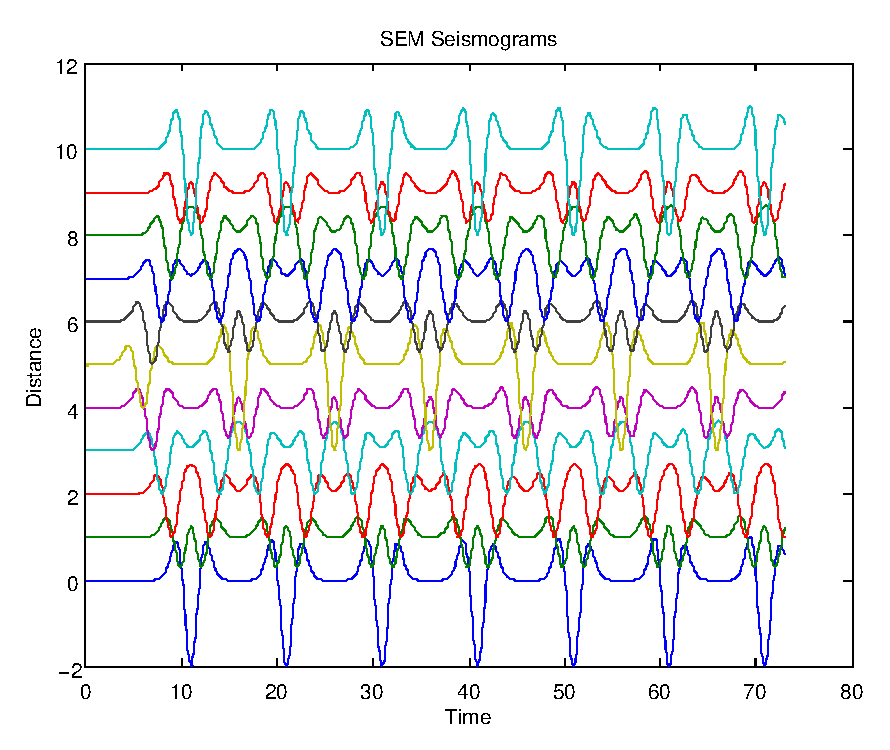
\includegraphics [width=4in]{sem1d_01.eps}



\end{document}
    
